\documentclass[conference]{IEEEtran}
\IEEEoverridecommandlockouts
\usepackage{cite}
\usepackage{amsmath,amssymb,amsfonts}
\usepackage{graphicx}
\usepackage{booktabs}
\usepackage{multirow}
\usepackage{xcolor}
\usepackage{siunitx}
\sisetup{detect-all}
\usepackage[hidelinks]{hyperref}
\usepackage{balance}

\newcommand{\Llay}{\mathcal{L}_{\mathrm{lay}}}
\newcommand{\Lflow}{\mathcal{L}_{\mathrm{flow}}}
\newcommand{\Lphoto}{\mathcal{L}_{\mathrm{photo}}}
\newcommand{\Laux}{\mathcal{L}_{\mathrm{aux}}}
\newcommand{\Cm}{\mathcal{C}}
\newcommand{\ours}{\textsc{Ours}}

\begin{document}

\title{Layout-Consistency Loss: Free Geometric\\Supervision for Document Image Dewarping}

\author{}

\maketitle

\begin{abstract}
Learned document dewarping is usually trained to regress a dense flow field with a pixel-wise loss, which treats every pixel error alike. Text, however, is hurt mostly by \emph{bending}: an error that varies along a text line curves it, while a rigid offset leaves it readable. We propose a layout-consistency loss that uses the region boxes that come free with layout datasets such as PubLayNet. Inside every text region, it penalizes the variance of the flow error along horizontal and vertical bands of the flat page. The loss is zero whenever the vertical error is constant within each horizontal band and the horizontal error within each vertical band, so it ignores rigid shifts and needs no OCR, line detector or flow inversion during training. We train a 6.45\,M-parameter U-Net flow regressor on 141{,}869 synthetic warps of PubLayNet pages, and run a controlled ablation in which the two arms differ only in this one loss weight. On the 2{,}737-sample validation set, the loss leaves flow end-point error unchanged (3.66 vs.\ 3.69\,px) while reducing our layout-distortion measure by 6.7\%. On a 334-page paired subset the reduction (6.1\%; 8.3\% for horizontal bending) is significant over pages ($p=1.5\times10^{-9}$), whereas the EPE difference is not ($p=0.59$). Tesseract character error rate on 332 re-rendered pages drops from 30.4\% to 28.6\% ($p=4.6\times10^{-6}$), and by 13.6\% relative on the hardest, photo-like warps. On the 130 real photographs of the DocUNet benchmark, which we evaluate with a protocol that reproduces published input scores, both arms improve clearly on the input. The two arms are statistically indistinguishable there, and both trail state-of-the-art methods trained on 3D-rendered or real data. Closing this real-photo gap is the main open problem.
\end{abstract}

\begin{IEEEkeywords}
document image dewarping, geometric rectification, layout analysis, optical flow, OCR
\end{IEEEkeywords}

%=====================================================================
\section{Introduction}
%=====================================================================
Photographs of paper documents are distorted by page curl, camera perspective and creases. Dewarping (also called unwarping or rectification) maps such a photo back to a flat page so that OCR and downstream document understanding work as they do on scans. Since DocUNet~\cite{ma2018docunet}, most learned methods regress a dense 2D mapping from the distorted image to the flat page~\cite{das2019dewarpnet,feng2021doctr,feng2022docgeonet,feng2024doctrpp,feng2025docscanner,verhoeven2023uvdoc}, and are supervised mainly with a pixel-wise loss on that mapping.

A pixel-wise flow loss is blind to \emph{how} an error is distributed. Consider two predictions with the same mean absolute flow error. In one, a whole text block is displaced by three pixels; in the other, the block's lines are bowed by a few pixels in the middle. Both cost the same under an $L_1$ flow loss, but only the second leaves curved text lines. Curved lines are a major cause of OCR errors and are what a reader perceives as ``not flat''.

Layout datasets already contain the information needed to tell these cases apart. PubLayNet~\cite{zhong2019publaynet} gives axis-aligned boxes for the text, title and list regions of more than 360K born-digital pages. In a correctly rectified page each such region must come out as an axis-aligned rectangle: its text lines horizontal and its margins vertical. We turn this property into a training loss.

\textbf{Contributions.}
\begin{itemize}
\item We propose a \emph{layout-consistency loss} $\Llay$. It measures the variance of the flow error within horizontal and vertical bands of text regions on the flat page. The loss ignores rigid shifts, so it targets bending and leaves global placement to the flow loss. It uses only box annotations, which are available for free when warps are synthesized from a layout dataset, and it requires no flow inversion during training (Sec.~\ref{sec:lay}).
\item We run a \emph{controlled single-variable ablation}: two 30-epoch training runs with identical data, seed, schedule and architecture, differing only in the weight of $\Llay$. We evaluate them on flow error, on layout distortion, and on OCR, with paired per-page statistics (Sec.~\ref{sec:exp}).
\item We give a \emph{reproducible real-photo evaluation} on the DocUNet benchmark. Our Octave/MATLAB pipeline and pinned Tesseract version reproduce the published input-image scores to within 0.004 MS-SSIM, 0.01 LD and 0.4\% ED (Setting~1), which makes our numbers directly comparable with prior work (Sec.~\ref{sec:docunet}).
\end{itemize}

The findings are mixed, and we report them as such. On synthetic data, $\Llay$ makes text geometry measurably straighter and OCR measurably better at no cost in average flow error. On real photographs, our models, trained only on 2D synthetic warps of born-digital pages, trail the state of the art by a wide margin, and there the effect of $\Llay$ is not detectable.

%=====================================================================
\section{Related Work}
%=====================================================================
\textbf{Learned dewarping.}
DocUNet~\cite{ma2018docunet} regresses a dense mapping with a stacked U-Net trained on synthetic 2D mesh perturbations and introduced the DocUNet benchmark. DewarpNet~\cite{das2019dewarpnet} rendered the Doc3D dataset from real paper meshes and predicts 3D coordinates before the backward map. Transformer-based models followed: DocTr~\cite{feng2021doctr} and DocTr++~\cite{feng2024doctrpp}, which handles unrestricted boundaries. DocScanner~\cite{feng2025docscanner} refines the flow progressively, and DocGeoNet~\cite{feng2022docgeonet} learns 3D shape and text-line representations. Other methods predict control points or grids: FDRNet~\cite{xue2022fdrnet}, DocReal~\cite{yu2024docreal} and UVDoc~\cite{verhoeven2023uvdoc}, the last of which also introduced line-straightness metrics. PaperEdge~\cite{ma2022paperedge} narrows the synthetic-to-real gap by training on real boundary-annotated photos, and Marior~\cite{zhang2022marior} removes margins and rectifies iteratively. DRNet~\cite{liu2024drnet} replaces ground-truth flow supervision with alignment to the flat image plus a self-consistency term. DocRes~\cite{zhang2024docres} handles dewarping among other restoration tasks. Classical methods reconstruct 3D shape~\cite{brown2001document} or optimize text-line and line-segment models~\cite{tian2011rectification,kim2015textline,kil2017robust}.

\textbf{Text-line, layout and straightness cues.}
Several works use content geometry, and their differences from ours are precise. DocGeoNet~\cite{feng2022docgeonet}, FTDR~\cite{li2023ftdr} and TextFlow~\cite{liu2026textflow} use text lines or text maps as \emph{auxiliary prediction targets or attention cues}. RDGR~\cite{jiang2022rdgr} enforces straight text lines in a \emph{per-image optimization at inference time}. LA-DocFlatten~\cite{li2024ladocflatten} segments layout primitives and regresses a \emph{separate local map per primitive}, which it merges into the global one. D2Dewarp~\cite{li2026d2dewarp} renders pages from PubLayNet and Chinese layout datasets and merges layout boundaries and OCR text lines into horizontal and vertical line masks, but uses them as \emph{segmentation targets and features}, not as a constraint on the flow. Two content-aware methods, like ours, place a geometric loss on the predicted flow. MataDoc~\cite{dai2023matadoc} constrains points on the same OCR-detected text line to share a $y$-coordinate. ForCenNet~\cite{cai2025forcennet} penalizes the difference in curvature of OCR text-box midlines and table lines between predicted and true flow. Content-agnostic straightness losses are also used: DocScanner's circle-consistency over all rows and columns~\cite{feng2025docscanner}, and the axis-aligned loss of~\cite{wang2026aadd}, which penalizes the variance of ground-truth coordinates along every row and column of the predicted grid; the latter is the closest in form to ours.

\emph{Our position.} We do not claim to be the first to use layout or text lines for dewarping. Our loss differs from the closest flow losses~\cite{dai2023matadoc,cai2025forcennet,wang2026aadd} as follows:
\begin{itemize}
\item it acts on \emph{2D regions} given by ground-truth layout boxes, not on 1D polylines from an OCR engine or line detector~\cite{dai2023matadoc,cai2025forcennet};
\item it restricts a row/column variance to \emph{text regions} while banding across the whole page, instead of applying it to every row and column of the grid~\cite{wang2026aadd};
\item its labels cost nothing when warps are synthesized from a layout dataset.
\end{itemize}
Our main contribution is the controlled measurement of what such a loss does, and does not, change.

%=====================================================================
\section{Method}
%=====================================================================
\begin{figure*}[t]
\centering
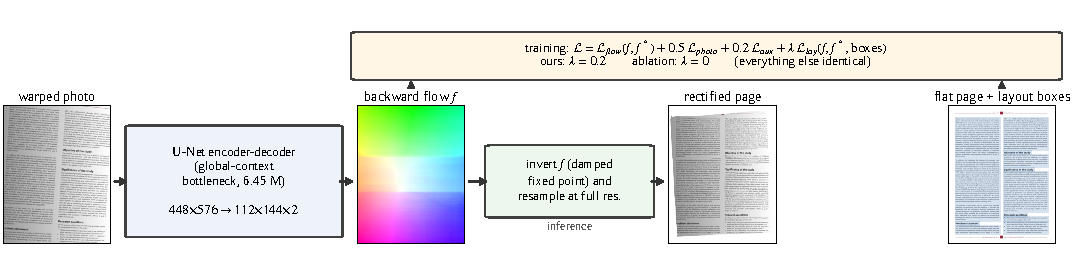
\includegraphics[width=\textwidth]{figs/pipeline.pdf}
\caption{Overview. A U-Net predicts a backward flow $f$ at quarter resolution from the distorted photo. During training, $f$ is compared with the true flow $f^*$, and the layout-consistency loss additionally uses the PubLayNet text-region boxes of the flat page. At inference, $f$ is upsampled, inverted by a damped fixed-point iteration and used to resample the photo once at full resolution. The two experimental arms differ only in $\lambda$.}
\label{fig:pipeline}
\end{figure*}

\subsection{Flow parameterization}
Fig.~\ref{fig:pipeline} gives an overview. Let $I_w$ be a distorted photo and $I_c$ the flat page, both $H\times W$. Following the convention used to generate our data, the network predicts a \emph{backward} displacement field $f$ defined on the distorted image,
\begin{equation}
I_w(\mathbf{p}) = I_c\big(\mathbf{p} + f(\mathbf{p})\big),
\label{eq:flow}
\end{equation}
so $c(\mathbf{p}) = \mathbf{p} + f(\mathbf{p})$ is the flat-page position of distorted pixel $\mathbf{p}$. Because the domain of $f$ is the input grid, every training loss can be computed in that domain without inverting the flow. Rectification needs the inverse map $g$, defined on the flat grid, with $I_c(\mathbf{q}) \approx I_w(\mathbf{q}+g(\mathbf{q}))$. We obtain $g$ at inference by the damped fixed-point iteration $g \leftarrow g + \beta\big(-f(\mathbf{q}+g) - g\big)$ with $\beta=0.5$ and 60 iterations. The undamped version ($\beta=1$) diverged on strongly compressive warps. Displacements are stored in normalized \texttt{grid\_sample} units~\cite{jaderberg2015stn}, so a prediction at any resolution can be applied to the full-resolution photo.

\subsection{Network}
The network is a U-Net~\cite{ronneberger2015unet} with five encoder stages (32 to 384 channels, BatchNorm and SiLU) on a $448\times576$ input. The input size keeps PubLayNet's US-Letter aspect ratio within 0.7\%. A global-context branch at the $14\times18$ bottleneck pools the features into a page-level vector and broadcasts it back, because curvature at one point of a page depends on geometry hundreds of pixels away. The decoder stops at $112\times144$, the resolution of the stored ground-truth flow, and a zero-initialized $3\times3$ head outputs $f$, so the network starts from the identity warp. Two auxiliary heads at $1/8$ and $1/16$ resolution provide deep supervision during training. The model has 6.45\,M parameters.

\subsection{Base objective}
The flow loss is a masked $L_1$ loss in pixels of the $448\times576$ page,
\begin{equation}
\Lflow = \frac{1}{2|M|}\sum_{\mathbf{p}\in M} \big\| D\,(f(\mathbf{p}) - f^*(\mathbf{p})) \big\|_1 ,
\end{equation}
where $M$ is the set of pixels that show the page (background pixels carry no meaningful flow) and $D$ converts normalized units to pixels. $\Laux$ is the same loss on the two auxiliary heads.

The photometric term resamples the flat page with the predicted flow and compares the result with the input. A naive version would mostly try to explain the synthetic shading with geometry: the raw difference between a perfectly resampled page and the shaded input is 45.3 grey levels. Since the shading is smooth by construction, both images are high-pass filtered (grey value minus a Gaussian blur, $\sigma=8$) before the $L_1$ comparison. The base objective is $\Lflow + 0.5\,\Lphoto + 0.2\,\Laux$.

\subsection{Layout-consistency loss}
\label{sec:lay}
Let $d(\mathbf{p}) = f(\mathbf{p}) - f^*(\mathbf{p})$ be the error field, and $c^*(\mathbf{p}) = \mathbf{p}+f^*(\mathbf{p})$ the true flat-page position. Take a horizontal text line inside a text region: all its pixels share the same $c^*_y$. After rectification with the predicted flow the line lands at $c^*_y + d_y$, so it stays straight \emph{if and only if $d_y$ is constant along it}. Any constant value of $d_y$ is a rigid vertical shift, which the flow loss already penalizes. The same argument applies to $d_x$ along a vertical margin.

We therefore partition the flat page into $B$ horizontal bands $\{\mathcal{H}_b\}$ and $B$ vertical bands $\{\mathcal{V}_b\}$ by the value of $c^*_y$ and $c^*_x$, respectively. Only pixels whose true flat-page position falls inside a layout region (text, title or list box) are kept:
\begin{equation}
R = \{\mathbf{p} \in M : c^*(\mathbf{p}) \in \textstyle\bigcup_k \mathrm{box}_k\}.
\end{equation}
The loss is $\Llay = \Cm_h + \Cm_v$, with
\begin{equation}
\begin{aligned}
\Cm_h &= \Big(\operatorname*{mean}_{b}\, \operatorname{Var}_{\mathbf{p}\in \mathcal{H}_b\cap R}\,[d_y(\mathbf{p})]\Big)^{1/2},\\
\Cm_v &= \Big(\operatorname*{mean}_{b}\, \operatorname{Var}_{\mathbf{p}\in \mathcal{V}_b\cap R}\,[d_x(\mathbf{p})]\Big)^{1/2},
\end{aligned}
\label{eq:lay}
\end{equation}
where bands holding fewer than 16 pixels are skipped and pixels are weighted by the (soft) page mask. $\Llay$ is computed on the $112\times144$ flow grid, so its unit is a grid pixel (four page pixels); the square root keeps it in length units, so that $\lambda=0.2$ corresponds to roughly 0.05 in the page-pixel units of $\Lflow$. We use $B=24$ bands, about 24 page pixels or a few text lines each. During training, the band statistics of all pages in a mini-batch are pooled before the square root (each page has its own bands); as an evaluation metric we compute it per page. Up to 32 regions per page are used, largest first.

Three properties follow.
\begin{itemize}
\item $\Llay=0$ if and only if $d_y$ is constant within every horizontal band and $d_x$ within every vertical band; in particular for $f=f^*$ and for any rigid shift.
\item Region membership is a box test on $c^*$, which comes directly from the stored flow, so no inversion is needed.
\item Bands are taken across the whole page, not per region. Two text blocks side by side at the same flat-page height are therefore constrained jointly, which is what keeps a two-column line of text level across the gutter.
\end{itemize}
Each band variance is computed with three scatter-adds, so apart from the box tests the cost does not depend on the number of regions. Fig.~\ref{fig:shiftbend} illustrates the shift invariance with the training code itself: a rigid shift and a bend with the same mean absolute error inside the text regions (3.00 grid px) give $\Llay=0.00$ and $2.68$, respectively. The full objective is $\Lflow + 0.5\Lphoto + 0.2\Laux + \lambda\Llay$; we use $\lambda=0.2$, and $\lambda=0$ for the ablation.

\begin{figure}[t]
\centering
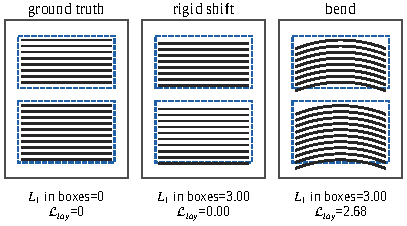
\includegraphics[width=\columnwidth]{figs/shift_bend.pdf}
\caption{Two text regions (dashed boxes) rectified with two erroneous flows whose mean absolute error inside the regions is equal ($L_1$, grid px). $\Llay$ (Eq.~\ref{eq:lay}, computed with our training code on the $112\times144$ grid) is zero for the rigid shift and large for the bend.}
\label{fig:shiftbend}
\end{figure}

%=====================================================================
\section{Synthetic Training Data}
%=====================================================================
\textbf{Source pages.} We use 47{,}958 PubLayNet~\cite{zhong2019publaynet} training pages (about one archive shard). We resize them to $448\times576$ and keep their region boxes. The 234 landscape pages (707 samples, 0.49\%) have no layout entries in our store and are excluded, leaving 144{,}606 samples.

\textbf{Warps.} Each page yields three samples, one per profile. Every warp contributes only a flow field; the flows are composed and the page is resampled once, which avoids cascaded interpolation blur.
\begin{itemize}
\item \emph{Cylinder}: a page bent around a cylinder (curl 0.15 to 0.85\,rad) seen by a pinhole camera at 1.6 to 4 page widths. It bows text lines toward the centre line, and the spine is horizontal in 25\% of samples.
\item \emph{Perspective}: a random homography whose corners move by up to $m$ of the page size, with $m$ drawn from 4 to 13\%.
\item \emph{Combined}: cylinder, perspective and a smooth random crease field (a $4\times4$ to $8\times8$ spline control grid, displacements up to 1 to 4\%), all always applied.
\end{itemize}
About 3\% of pages also get a \emph{flat} sample (no page deformation, camera framing only) so that the model learns to leave flat pages alone.

\textbf{Framing and appearance.} A random camera framing is composed with every warp: a tight crop (scale 1.02 to 1.3, roll up to $\pm5^\circ$), exact framing, or a pulled-back shot (scale 0.7 to 0.98, roll up to $\pm7^\circ$). Without it, the fraction of the frame covered by the page was strongly correlated with warp magnitude ($r=-0.79$), a shortcut a network could exploit. The page is composited on a synthetic surface, 22\% of which are near-white, and given a soft contact shadow. Smooth shading gradients are applied to 75\% of the samples. Images are stored as JPEG (quality 90), and flows and masks at $112\times144$ (flow storage error 0.02\,px).

\textbf{Split.} Train and validation are split by \emph{page}, using an MD5 hash of the page identifier, so that the variants of one page never straddle the split. This gives 141{,}869 training and 2{,}737 validation samples (901 cylinder, 901 perspective, 901 combined, 34 flat).

%=====================================================================
\section{Experiments}
\label{sec:exp}
%=====================================================================
\subsection{Setup}
Both arms are trained for 30 epochs (531{,}990 steps, batch 8) with AdamW~\cite{loshchilov2019adamw} (learning rate $3\times10^{-4}$, weight decay $10^{-4}$), 500 warm-up steps and cosine decay~\cite{loshchilov2017sgdr} over 540{,}000 steps. They use mixed precision~\cite{micikevicius2018mixed} on a single NVIDIA T4, at 8.6 (layout arm) and 9.2 (ablation) steps/s, i.e.\ 16 to 18\,h per run. Each run spans two sessions with exact checkpoint resumption (restored state verified bit-exact in a CPU test). The arms use the same code, data, split and random seed (1234), and differ only in $\lambda\in\{0.2, 0\}$. We train one seed per arm; Sec.~\ref{sec:limits} discusses this.

\textbf{Metrics.}
\begin{itemize}
\item \emph{EPE}: the end-point error of the predicted flow, in pixels of the $448\times576$ page, over page pixels.
\item \emph{Layout distortion $\Cm = \Cm_h + \Cm_v$}: Eq.~(\ref{eq:lay}) evaluated per page as a metric, on the $112\times144$ grid (one unit is four page pixels), and averaged over pages. Lower values mean straighter text regions. It is computed offline from each checkpoint for both arms, since the ablation never computes it during training.
\item \emph{OCR} and DocUNet metrics are described with their experiments below.
\end{itemize}
Paired tests compare the two arms on the same pages (differences are taken as ablation minus ours, so positive values favour ours): two-sided Wilcoxon signed-rank tests~\cite{wilcoxon1945individual} and 95\% percentile-bootstrap confidence intervals~\cite{efron1993bootstrap} (10{,}000 resamples). These capture variation over pages, not over training runs.

\subsection{Flow error and layout distortion}
\begin{table}[t]
\centering
\caption{Synthetic validation results at step 531{,}990. Top: full validation set ($n=2{,}737$; per-page $\Cm_h,\Cm_v$ were only computed on the subset). Bottom: per-page paired comparison on the 334-page OCR subset (Sec.~\ref{sec:ocrsyn}). ``Red.'' is the relative reduction of the ablation's value achieved by our arm, with its 95\% bootstrap CI.}
\label{tab:synth}
\setlength{\tabcolsep}{3pt}
\begin{tabular}{@{}lcccc@{}}
\toprule
 & EPE (px)\,$\downarrow$ & $\Cm$\,$\downarrow$ & $\Cm_h$\,$\downarrow$ & $\Cm_v$\,$\downarrow$ \\
\midrule
Identity (no dewarping) & 39.88 & -- & -- & -- \\
Ablation ($\lambda=0$) & 3.689 & 0.4714 & -- & -- \\
\ours{} ($\lambda=0.2$) & \textbf{3.662} & \textbf{0.4398} & -- & -- \\
Reduction & 0.7\% & 6.7\% & -- & -- \\
\midrule
\multicolumn{5}{@{}l}{\emph{Paired, 334 pages}} \\
Red. [95\% CI] & \begin{tabular}[c]{@{}c@{}}1.9\%\\{}[$-$1.6, 5.6]\end{tabular} & \begin{tabular}[c]{@{}c@{}}6.1\%\\{}[4.1, 8.2]\end{tabular} & \begin{tabular}[c]{@{}c@{}}8.3\%\\{}[5.6, 11.1]\end{tabular} & \begin{tabular}[c]{@{}c@{}}3.8\%\\{}[0.8, 6.8]\end{tabular} \\
Pages better / worse & 160 / 174 & 214 / 120 & 219 / 114 & 187 / 147 \\
Wilcoxon $p$ & 0.59 & $1.5{\times}10^{-9}$ & $3.5{\times}10^{-10}$ & $4.9{\times}10^{-3}$ \\
\bottomrule
\end{tabular}
\end{table}

Table~\ref{tab:synth} shows the central result. Both arms reduce the flow error by about 91\% relative to the identity mapping, and their EPEs differ by 0.7\%. On the paired subset, the EPE difference is not significant ($p=0.59$; the arm with $\Llay$ is better on fewer pages than it is worse). The layout distortion, by contrast, is 6.7\% lower with $\Llay$ on the full validation set; on the paired subset the reduction (6.1\%) is significant over pages ($p=1.5\times10^{-9}$), with lower $\Cm$ on 214 of 334 pages. The effect is largest for horizontal bending ($\Cm_h$, 8.3\%), which is what curves text lines. In other words, $\Llay$ redistributes the error rather than shrinking it: for about the same amount of error, less of it is within-band variation, i.e.\ bending.

Fig.~\ref{fig:profiles} breaks the result down by warp profile. The reduction in $\Cm$ is consistent across the three warped profiles, at 6.2\% (cylinder), 6.7\% (perspective) and 6.9\% (combined) on the full validation set, while the EPE differences stay within $\pm$1.5\%. For the 34 flat samples, the differences in both EPE and $\Cm$ lie within the noise.

\begin{figure}[t]
\centering
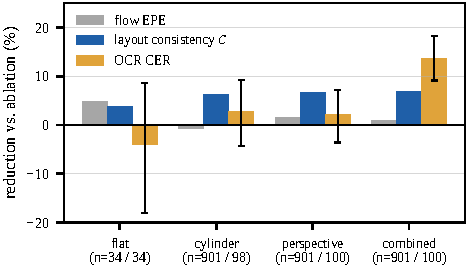
\includegraphics[width=\columnwidth]{figs/profiles.pdf}
\caption{Relative reduction (ablation $\to$ ours) per warp profile. EPE and $\Cm$ are from the full validation set, OCR CER from the 332-page OCR test; the bars show 95\% bootstrap CIs for OCR. Sample counts are given as validation / OCR.}
\label{fig:profiles}
\end{figure}

\textbf{Training dynamics.} Fig.~\ref{fig:curves} shows validation EPE throughout training on a fixed 480-sample monitoring subset, which is evaluated every 1{,}000 steps at identical steps for both arms. The arms track each other closely throughout. On this subset the EPE gap settles at about 4\% in favour of ours; on the full validation set it is 0.7\%. We therefore do not claim an EPE improvement. An intermediate full-validation evaluation also points the same way: for the validation-selected checkpoints of each arm's first training session (step 341{,}000, 19.2 epochs, for ours; step 326{,}000, 18.4 epochs, for the ablation), the EPE gap was 3.9\% and the $\Cm$ gap 7.8\%. During the final learning-rate anneal the EPE gap almost closed, while the $\Cm$ gap persisted. (These two checkpoints are 0.85 epochs apart, with ours trained longer, and were selected on validation, so we report them only as an indication.)

\begin{figure}[t]
\centering
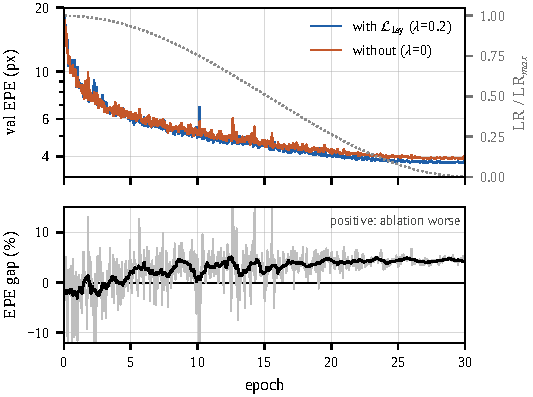
\includegraphics[width=\columnwidth]{figs/curves.pdf}
\caption{Validation EPE of both arms over training (fixed 480-sample monitoring subset, evaluated every 1{,}000 steps), with the cosine learning-rate schedule (dotted). Bottom: relative EPE gap; light: raw, dark: rolling mean over 15 evaluations.}
\label{fig:curves}
\end{figure}

\subsection{OCR on synthetic pages}
\label{sec:ocrsyn}
\textbf{Protocol.} At $448\times576$ the text of a PubLayNet page is too small to read reliably: even rectification with the \emph{true} flow gave a 66 to 71\% character error rate in a pilot test. We therefore re-synthesize each page at $3\times$ resolution:
\begin{enumerate}
\item the flat page is upsampled ($1344\times1728$, bicubic) and warped with its ground-truth flow, which gives the \emph{input};
\item each model predicts its flow from the original stored $448\times576$ photo (its training input);
\item the predicted flow is upsampled, inverted, and applied to the $3\times$ input;
\item the true flow, applied the same way, gives an upper bound.
\end{enumerate}
The pages are a fixed, stratified validation subset chosen by a seeded hash of the page ID before any OCR was run: 100 pages each of cylinder, perspective and combined, plus all 34 flat. Two pages whose reference has fewer than 200 characters are dropped, leaving 332. Text is read with Tesseract~5.3.4 (LSTM engine, \texttt{--oem 1 --psm 3})~\cite{smith2007tesseract}, and whitespace is normalized. The reference is Tesseract's reading of the flat $3\times$ page. CER is the edit distance divided by the reference length.

\begin{table}[t]
\centering
\caption{OCR character error rate (\%) on 332 synthetic validation pages re-rendered at $3\times$ (lower is better). ``Combined'' is the hardest, most photo-like profile ($n=100$). Paired differences are ablation minus ours (positive favours ours), with 95\% bootstrap CIs.}
\label{tab:ocr}
\setlength{\tabcolsep}{5pt}
\begin{tabular}{@{}lcccc@{}}
\toprule
 & \multicolumn{3}{c}{All pages ($n=332$)} & Combined \\
\cmidrule(lr){2-4}\cmidrule(l){5-5}
 & mean & corpus & median & mean \\
\midrule
Input (no dewarping) & 63.05 & 62.82 & 71.17 & 77.01 \\
Ablation ($\lambda=0$) & 30.37 & 24.55 & 21.69 & 34.47 \\
\ours{} ($\lambda=0.2$) & \textbf{28.61} & \textbf{22.82} & \textbf{20.52} & \textbf{29.78} \\
True flow (upper bound) & 13.70 & 9.92 & 7.03 & 18.19 \\
\midrule
Paired diff.\ (pts) & \multicolumn{3}{c}{$+1.76$ [0.78, 2.79]} & $+4.69$ [2.95, 6.62] \\
Pages better / worse & \multicolumn{3}{c}{203 / 126 (3 ties)} & 74 / 25 \\
Wilcoxon $p$ & \multicolumn{3}{c}{$4.6\times10^{-6}$} & $4.9\times10^{-7}$ \\
\bottomrule
\end{tabular}
\end{table}

\textbf{Results.} Table~\ref{tab:ocr} shows that dewarping roughly halves the input CER, and that the arm trained with $\Llay$ reads better. Its mean CER is 1.76 points (5.8\% relative) lower than the ablation's, and it wins on 203 of 332 pages ($p=4.6\times10^{-6}$). Measured by the share of the possible gain realized (from input to the true-flow bound), the arms reach 69.8\% and 66.2\%. The gain is concentrated on the combined profile: there CER drops from 34.5\% to 29.8\% (13.6\% relative), with 74 wins against 25. On the other three profiles together, the difference ($+0.50$ points, $p=0.056$) is not significant (Fig.~\ref{fig:profiles}). While the relative $\Cm$ reduction is similar across profiles, its absolute size is largest on combined warps (0.052 grid px, vs.\ 0.018 and 0.026 for cylinder and perspective). A plausible explanation, which we have not tested directly, is that mild warps leave nearly straight lines in both arms, while on compound warps the remaining bending is large enough to affect recognition.

Fig.~\ref{fig:synthqual} shows the first page of each profile in the hash-ordered subset. The images were not selected by result.

\begin{figure*}[t]
\centering
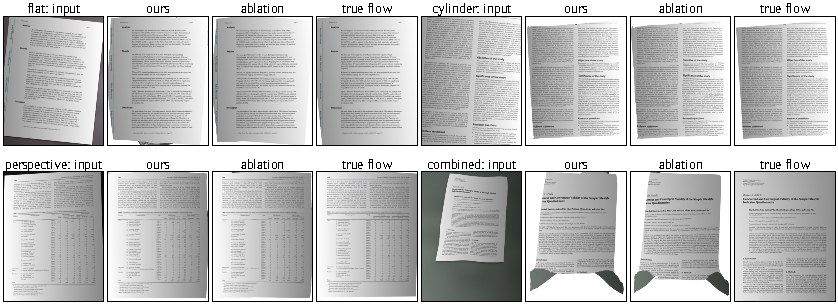
\includegraphics[width=\textwidth]{figs/synth_qual.pdf}
\caption{Synthetic validation examples: the first page of each profile in the OCR subset, which was fixed before any OCR was run (not selected by result). Each group shows the stored input photo, the rectifications of both arms, and the rectification with the true flow (which retains the synthetic shading). Pixels whose source lies outside the photo are filled white. The combined example shows a typical failure of \emph{both} arms: the lower page corners are underestimated and background is pulled in.}
\label{fig:synthqual}
\end{figure*}

\subsection{Real photographs: DocUNet benchmark}
\label{sec:docunet}
\textbf{Protocol.} The DocUNet benchmark~\cite{ma2018docunet} contains 130 phone photos of 65 paper documents with flatbed scans as ground truth. We apply both final models to the benchmark's standard crops without any fine-tuning, further cropping or background removal. Each photo is resized to $448\times576$ for the network; the predicted flow is upsampled to the photo's full resolution, inverted there, and used to resample the photo once, with white fill outside the image. We follow the evaluation code released with DocTr and its successors~\cite{feng2021doctr,feng2022docgeonet,feng2025docscanner,feng2024doctrpp}:
\begin{itemize}
\item DocUNet-style \emph{MS-SSIM}~\cite{ma2018docunet,wang2003msssim} (weighted sum of SSIM over a 5-level pyramid) and \emph{Local Distortion} (LD, mean SIFT-flow~\cite{liu2011siftflow} displacement) on grey images, with the scan resized to an area of 598{,}400 pixels and the result resized to the scan's size;
\item \emph{ED/CER}: edit distance and character error rate of default-parameter \texttt{pytesseract} output against the scan's OCR, on the 60-image (``Setting~1'', DocTr) and 50-image (``Setting~2'', DewarpNet) text-rich subsets;
\item the corrected benchmark, in which document 64 is rotated by $180^\circ$.
\end{itemize}

\textbf{Reproducing published scores.} We had no MATLAB, so we ran the original evaluation code in GNU Octave 8.4 with its \texttt{image} package (2.14). This required compiling the SIFT-flow MEX files for Octave and adding a MATLAB-compatible \texttt{ssim}. ED/CER are sensitive to the OCR engine, so we built Tesseract 5.0.1 from source, the version used for the published scores (with the standard English model of the Ubuntu \texttt{tesseract-ocr-eng} 4.1 package). As Table~\ref{tab:docunet} shows, our score for the unrectified inputs (``Distorted'' row) matches the published one. MS-SSIM is 0.249 vs.\ 0.246, LD 20.52 vs.\ 20.51, ED (Setting~1) 1546.5 vs.\ 1552.2 and CER 0.509 vs.\ 0.509. Setting~2 (2092.8/0.531 vs.\ 2111.6/0.535) is also close. Our numbers can therefore be compared with the published ones. With the newer Tesseract 5.3.4, the input CER drops to 0.484, which shows how much the engine version matters.

\begin{table}[t]
\centering
\caption{DocUNet benchmark (130 real photos, corrected; Tesseract 5.0.1 for ED/CER, Settings 1 / 2 use 60 / 50 images). Rows marked $\dagger$ are published values~\cite{feng2022docgeonet,feng2025docscanner}; the remaining rows were computed by us with the same protocol. $\ddagger$: trained on Doc3D (3D-rendered) data and/or real photos.}
\label{tab:docunet}
\footnotesize\setlength{\tabcolsep}{1.8pt}
\begin{tabular}{@{}lcccccc@{}}
\toprule
 & MS-SSIM$\uparrow$ & LD$\downarrow$ & ED$_1\downarrow$ & CER$_1\downarrow$ & ED$_2\downarrow$ & CER$_2\downarrow$ \\
\midrule
Distorted$^\dagger$ & 0.246 & 20.51 & 1552.2 & 0.509 & 2111.6 & 0.535 \\
Distorted (our repro.) & 0.249 & 20.52 & 1546.5 & 0.509 & 2092.8 & 0.531 \\
\midrule
DocUNet$^\dagger$~\cite{ma2018docunet} & 0.410 & 14.19 & 1259.8 & 0.397 & 1933.7 & 0.463 \\
DewarpNet$^{\dagger\ddagger}$~\cite{das2019dewarpnet} & 0.474 & 8.39 & 525.5 & 0.210 & 885.9 & 0.237 \\
DocTr$^{\dagger\ddagger}$~\cite{feng2021doctr} & 0.511 & 7.76 & 464.8 & 0.175 & 724.8 & 0.183 \\
DocGeoNet$^{\dagger\ddagger}$~\cite{feng2022docgeonet} & 0.504 & 7.71 & 379.0 & 0.151 & 713.9 & 0.182 \\
PaperEdge$^{\dagger\ddagger}$~\cite{ma2022paperedge} & 0.472 & 7.99 & 375.6 & 0.154 & 777.8 & 0.201 \\
DocScanner-L$^{\dagger\ddagger}$~\cite{feng2025docscanner} & 0.518 & 7.45 & 390.4 & 0.149 & 632.3 & 0.165 \\
\midrule
Ablation ($\lambda=0$) & 0.322 & 16.85 & 1081.1 & 0.390 & 1513.8 & 0.395 \\
\ours{} ($\lambda=0.2$) & 0.324 & 16.98 & 1061.4 & 0.363 & 1555.9 & 0.406 \\
\bottomrule
\end{tabular}
\end{table}

\textbf{Results.} Both arms improve substantially on the input. MS-SSIM rises from 0.249 to 0.32, LD falls from 20.5 to about 17, and CER falls from 0.51 to 0.36--0.39 (Setting~1). Per image, MS-SSIM improves on 78\% (ours) and 82\% (ablation) of the photos. The two arms are statistically indistinguishable on real photos. The paired differences (ours minus ablation; 95\% CIs resample documents, Wilcoxon tests treat the 130 or 60/50 images as independent) are:
\begin{itemize}
\item MS-SSIM $+0.002$ [$-0.005$, $0.009$], $p=0.55$;
\item LD $+0.13$ [$-0.47$, $0.75$], $p=0.66$;
\item CER, Setting~1: $-0.027$ [$-0.072$, $0.011$], $p=0.19$;
\item CER, Setting~2: $+0.011$ [$-0.041$, $0.059$], $p=0.67$.
\end{itemize}
With Tesseract 5.3.4 the Setting~1 difference becomes significant ($0.344$ vs.\ $0.384$, $p=0.015$) while Setting~2 does not ($p=0.44$). Because this conclusion depends on the OCR engine, we do not claim a real-photo OCR gain.

\begin{figure*}[t]
\centering
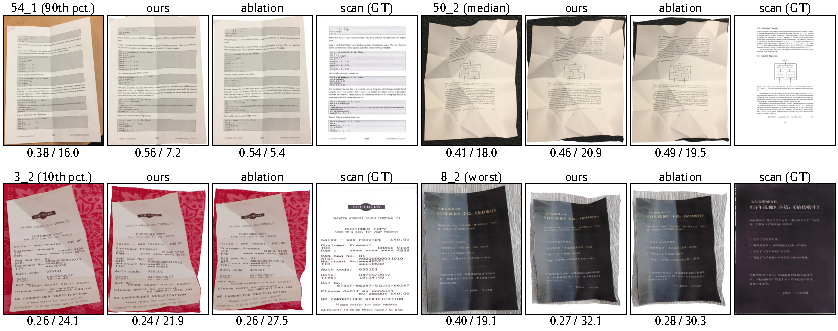
\includegraphics[width=\textwidth]{figs/docunet_qual.pdf}
\caption{DocUNet results, selected by rule: the photos at the 90th, 50th and 10th percentile of our MS-SSIM gain over the input, and the worst one. Numbers give MS-SSIM / LD. Visible problems include crumpling that our smooth synthetic creases do not model (50\_2), a strongly textured background with a narrow receipt (3\_2), and background pulled into the output of a dark page (8\_2).}
\label{fig:docunetqual}
\end{figure*}

Compared with prior work, our models obtain lower ED and CER than the original DocUNet (by a small margin for the ablation in Setting~1), but lower MS-SSIM and higher LD, and they are far behind methods trained on Doc3D or real photos. We did not isolate the cause; Fig.~\ref{fig:docunetqual} illustrates likely failure modes. Our synthetic warps are smooth (a cylinder, a homography and a low-frequency crease field), whereas many benchmark documents are folded or crumpled. The page boundary is often misjudged on cluttered or patterned backgrounds, which leaves background in the output and is heavily penalized by MS-SSIM. Our pages are exclusively born-digital English scientific articles, while the benchmark includes receipts, posters, magazines and Chinese text. Architecture and input resolution may also play a role: DocUNet, likewise trained on 2D synthetic warps, scores higher on MS-SSIM and LD. Against errors of this size, a loss that refines the straightness of already well-localized text regions has little room to show an effect.

%=====================================================================
\section{Discussion and Limitations}
\label{sec:limits}
%=====================================================================
\textbf{What the evidence supports.} Holding everything else fixed, adding $\Llay$ changes the \emph{shape} of the flow error. Text regions come out measurably straighter, especially in the horizontal direction, while the average error stays the same. On synthetic pages this translates into better OCR, concentrated on the hardest warps. The loss adds two scatter-based band variances per batch, and its labels come for free when warps are synthesized from a layout dataset.

\textbf{Limitations.}
\begin{enumerate}
\item \emph{One seed per arm.} The confidence intervals reflect variation over pages, not over training runs. Each run took about 17 GPU-hours on the free hardware available to us. Repeating the ablation over several seeds is the most important next step.
\item \emph{Our own metric.} $\Cm$ is the quantity that $\Llay$ optimizes. We therefore also report OCR, which is not, but OCR uses a synthetic reference: Tesseract's reading of the flat page, not human transcriptions.
\item \emph{Synthetic OCR rendering.} OCR used $3\times$ re-rendering, with inputs that lack the synthetic shading and background seen by the models.
\item \emph{Real photos.} On DocUNet both arms are far from the state of the art, and we have not determined how much of this is due to the training data, the architecture or the input resolution. Combining $\Llay$ with Doc3D-style 3D renderings, real-photo fine-tuning~\cite{ma2022paperedge} or stronger crease models is the natural way to test whether the synthetic gains transfer.
\item \emph{Rectangular regions.} The loss assumes axis-aligned rectangular regions, which holds for born-digital layouts but not for rotated or free-form content.
\end{enumerate}

%=====================================================================
\section{Conclusion}
%=====================================================================
We introduced a layout-consistency loss that uses free layout-box annotations to penalize the bending of text regions in a predicted dewarping flow, while ignoring rigid shifts. In a controlled single-variable ablation, it lowered layout distortion by 6.7\% and synthetic-page OCR error by 5.8\% (13.6\% on the hardest warps), at no cost in flow end-point error. On real DocUNet photos both arms clearly improve on the input, but the difference between them is not detectable, and both remain well behind methods trained on 3D-rendered or real data. We release our evaluation setup, which reproduces published DocUNet input scores in Octave, to make such comparisons easy to repeat.

\bibliographystyle{IEEEtran}
\bibliography{refs}

\end{document}
